\documentclass[12pt,letterpaper,noanswers]{exam}
\usepackage[usenames,dvipsnames,svgnames,table]{xcolor}
\usepackage[margin=0.9in]{geometry}
\renewcommand{\familydefault}{\sfdefault}
\usepackage{multicol}
\pagestyle{head}
\header{AM 111 Class 19}{}{Initial value problems: differential equations, p.\thepage}
\runningheadrule
\headrule
\usepackage{siunitx}
\usepackage{graphicx} % more modern
\usepackage{amsmath} 
\usepackage{amssymb} 
\usepackage{hyperref}
\usepackage{tcolorbox}
\usepackage{enumitem}
\def\mbf{\mathbf}
\newcommand{\vc}[1]{\boldsymbol{#1}}
\def\dsst{\displaystyle}
\DeclareMathOperator*{\argmin}{arg\,min} % thin space, limits underneath in displays
\usepackage{listings}

\begin{document}
 \pdfpageheight 11in 
  \pdfpagewidth 8.5in

\noindent 

\section*{Preliminaries}

\begin{itemize}
\itemsep0pt
\item Problem set 08 is due Friday
\item There is a skill check in the next class.
\item A project log is due on Friday as part of the problem set.
\end{itemize}


\noindent\textbf{Big picture}

Today: Approximating solutions to equations that can be written in the form \[\displaystyle\left\{\begin{array}{l}\dfrac{dy}{dt} = f(y(t),t) \\
\\
y(a) = y_a\end{array}\right.\]

\vspace{0.2cm}
\hrule
\vspace{0.2cm}

\noindent \textbf{Skill check practice}

\item Consider the initial value problem $\left\{\begin{array}{l}
y' = -2y \\
y(-2) = 5
\end{array}
\right.$

Set $h = 0.1$.  Provide an expression for $y(-2+0.1)$, as approximated using improved Euler/ trapezoid.




\vspace{0.2cm}
\hrule
\vspace{0.2cm}

\noindent \textbf{Skill check solution}

Answer: $5 + 0.1 \frac{1}{2}(f(-2,5) +f(-1.9,4)) = 5+0.1(-10-8)/2 = 4.1$

More steps:

Explicit trapezoid:
$w_0 = y_0$, $w_1 = w_0 + \frac{h}{2}\left(f(t_0,w_0) + f\left(t_0+h, w_0 + hf(t_0,w_0)\right)\right)$


In Euler's method, $w_0 = 5$, $w_1 = 5 + 0.1f(-2,5) = 5+0.1(-10) = 4$.

$f(-1.9,4) = -8$

For explicit trapezoid, use $w_0 + 0.1 \frac{1}{2}(f(-2,5) +f(-1.9,4)) = 5+0.1(-10-8)/2$.

\emph{Explicit trapezoid gives $4.1$ while Euler gives $4$.}

\vspace{0.2cm}
\hrule
\vspace{0.2cm}



\section*{Ordinary differential equations}
\subsection*{Initial value problems (See Sauer \S 6.1}

\begin{enumerate}[resume=classQ]
\item The \textbf{logistic model} for population is given by $\dfrac{dy}{dt} - cy(1-y) = 0$ with  $y(0) = y_0$.  What steps are involved to use substitution to show that $y(t) = 1 - \left(1-\dfrac{y_0}{1-y_0}e^{ct}\right)^{-1}$ satisfies the equation?
\vspace{1in}
\item Consider the differential equation $y'' + 3y'(t) - y = 0$.  What is the order of this equation?
\vspace{1cm}
\end{enumerate}

\begin{enumerate}[resume=classQ]
\item For a slope field of $dy/dx = f(x,y)$, a short line segment with slope $f(x,y)$ is drawn at a selection of points $(x,y)$.
\begin{parts}
\item When will the slope be the same at every point on a vertical line?  When will it be the same at every point on a horizontal line?
\vspace{0.5in}
\item The slope $dy/dx$ will be tangent to a solution curve $y(x)$ at every point on the curve.  Use this fact about tangents to sketch a solution curve that starts at $y(-2) = 1$ for each of the slope fields below.
\end{parts}

\hspace{-1in}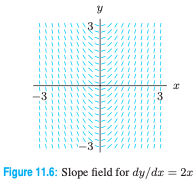
\includegraphics[width=0.4\linewidth]{img/C18-HHslopefield.png}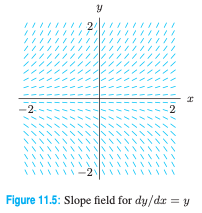
\includegraphics[width=0.33\linewidth]{img/C18-HHslope2.png}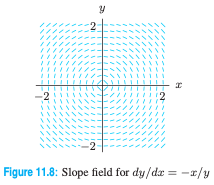
\includegraphics[width=0.4\linewidth]{img/C18-HHslope3.png}
\end{enumerate}

\begin{enumerate}[resume=classQ]
\item Let $dy/dt = cy$, $y(0) = y_0$, and $t\in[0,1]$.
\begin{parts}

\item Find an expression for $w_1$ in terms of $y_0, c, h$, and then an expression for $w_k$ in terms of $y_0, c, h$ to find the approximation by Euler's method.
\vspace{1in}

\item For this differential equation we are able to find an exact solution.  Substitute into $dy/dt - cy$ to show that $y(t) = y_0e^{ct}$ is an exact solution to this IVP.
\vspace{1in}

\end{parts}
Fix $t$ and use $n$ steps, so that $h = t/n$.  You should find that $w_n = y_0(1+ct/n)^n$.  In the limit as $n\rightarrow\infty$ this is $y_0e^{ct}$, so Euler's method converges to the correct value.
\end{enumerate}

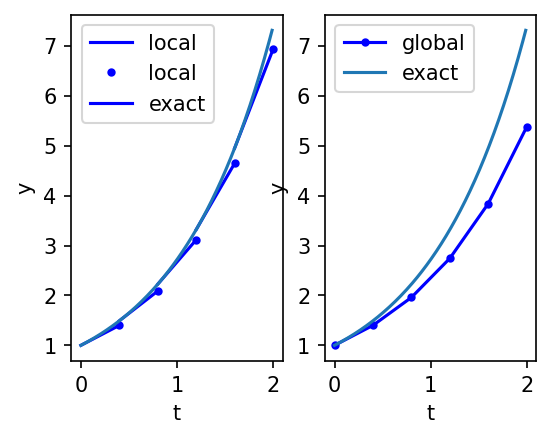
\includegraphics[]{img/C18Euler.png}
\begin{enumerate}[resume=classQ]
    \item Examine the error plots above for a solution to an initial value problem.
    \begin{parts}
    \item Estimate $h$.
    \item How do the lines labeled 'local' show local truncation error?  How does the curve labeled 'global' show global truncation error?
    \vspace{1cm}
    \end{parts}
\item Find the local truncation error for Euler's method using Taylor expansion.
\begin{parts}
\item Assume $w_k$ is the exact value of $y(t_k)$. Taylor expand $y(t_{k+1}) = y(t_k+h)$ to first order about $y(t_k)$, and then include the remainder term (2nd order).
\vspace{1in}
\item Euler's method sets $w_{k+1} = w_k + hf(t_k,w_k)$.  Find $\vert w_{k+1} - y(t_{k+1})\vert$ to find the local truncation error.  \emph{It you have Taylor expanded correctly, it should be set by the remainder term.}
\vspace{1cm}
\end{parts}
For $M$ an upper bound on $y''$ on $[a,b]$ the local truncation error satisfies $e_k \leq Mh^2/2$
\end{enumerate}


\begin{enumerate}[resume=classQ]
    \item (explicit trapezoid) In Euler's method, $w_{k+1} = w_k + hf(t_k, w_k)$.
    \begin{parts}
    \item $f(t_k, w_k)$ is an estimate of the slope of the interval $[t_k, t_{k+1}]$and $f(t_{k+1}, w_{k+1})$ is a second estimate.  Write down a rule that uses the average of these for its approximation of the slope over the interval.
    \vspace{1in}
    
    \emph{This is a two stage method.  This method is called improved Euler, trapezoid method, or Heun method.}
    \item To identify the local truncation error, start by Taylor expanding $f(t_k + h, w_k+hf(t_k,w_k)$ about $(t_k, w_k)$.  It is sufficient to expand to first order (following the format below).
    
    \emph{To do a 2D Taylor expansion to first order, $f(t+h, y + \Delta) \approx f(t,y) + h\dfrac{\partial f}{\partial t}(t,y) + \Delta \dfrac{\partial f}{\partial y}(t,y) + \mathcal{O}(h^2)$ (for the dropped terms to be $\mathcal{O}(h^2)$, I am assuming that $\Delta$ is $\mathcal{O}(h)$).}
    \vspace{1in}
    
    \item The local truncation error is $\vert y_{k+1} - w_{k+1}\vert$ (after assuming that $w_k = y_k$).  Do this subtraction to show that it is $\mathcal{O}(h^3)$.
    \vspace{1in}
    \end{parts}
    \item The global error for improved Euler will be $\mathcal{O}(h^2)$ so it is said to be a second order method (while Euler is a first order method).  How can you tell the order of the methods in the plot of error below?  What happens to the error from improved Euler as step size becomes small (and why)?
\end{enumerate}


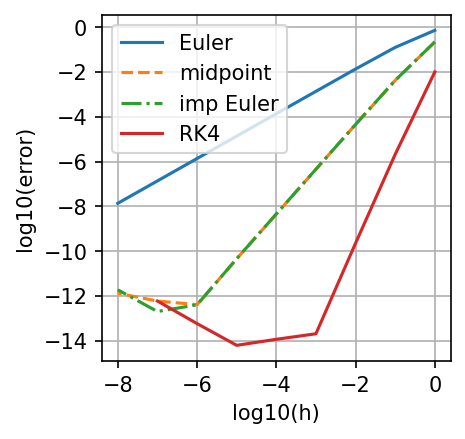
\includegraphics[]{img/C18error.png}
\subsection*{Systems of first order equations}

\begin{enumerate}[resume=classQ]
\item Convert the second-order differential equation $y'' = a(y')^2 +yy' - \cos t$ to a system of two first order equations.
\begin{parts}
\item Set $y_1 = y$ and define the new variable $y_2 = y'$.  Rewrite the equation above, by replacing $y''$ with $y_2'$.  Replace $y'$ with $y_2$.  Replace $y$ with $y_1$.
\vspace{1cm}
\item Write down your system.  $y_1' = y_2$ is the first equation in the system.  $y_2' = ??$ is the second equation.
\vspace{1.5cm}
\end{parts}
\item Apply one step of Euler's method to initial value problem \[\left\{\begin{array}{l}
y_1' = y_2 - y_1^2 \\
y_2' = y_1 -ty_2^3 \\
y_1(1) = 0 \\
y_2(1) = 3 \end{array}\right.\]
$\begin{array}{l}
w_{0,1} = 0\\
w_{0,2} = 3
\end{array}$. Set up expressions for $\begin{array}{l}
w_{1,1}\\
w_{1,2}
\end{array}$
\vspace{1in}
\end{enumerate}

\end{document}